\documentclass{article}
\usepackage[utf8]{inputenc}
\usepackage{amssymb}
\usepackage{amsmath}
\usepackage{bbold}
\usepackage{graphicx}
\usepackage{multirow}

\title{Note on Induced Norms}
\author{Thomas Maierhofer}
\date{\today}

\begin{document}

\newcommand{\Prob}{\mathbb{P}}
\newcommand{\V}{\mathbb{V}}
\newcommand{\Cov}{\text{Cov}}
\newcommand{\E}{\mathbb{E}}
\newcommand{\R}{\mathbb{R}}
\newcommand{\1}{\mathbb{1}}
\newcommand{\LL}{\mathcal{L}}
\newcommand{\F}{\mathcal{F}}
\newcommand{\iid}{\overset{\text{iid}}{\sim}}
\newcommand{\SUM}{\sum_{i=1}^n}
\newcommand{\PROD}{\prod_{i=1}^n}

\maketitle

\section{Background: $p$ Norms for Vectors}
This section formally introduces $p$ norms with a focus on the special cases $ p = 0, 1, 2, \infty$.
The $p$ norm of a vector $x \in \R^d$ is denoted as $||x||_p$ and defined as
$$||x||_p = \left(\sum_{i = 1}^d |x_i|^p \right)^{1/p},$$
where $|x_i| = \text{sign}(x_i)x_i$ denotes the absolute value. In literature $p$ norms are often denoted as $l_p$ norms.

The most important special cases is the $2$ norm, a.k.a.\ Euclidean norm. It is defined as
$$||x||_2 = \sqrt{\sum_{i = 1}^d x_i^2}.$$
Other important cases include the $0$ norm,
$$||x||_0 = \sum_{i = 1}^d \1\{x_i \neq 0\},$$
the $1$ norm, a.k.a.\ Manhattan norm,
$$||x||_1 = \sum_{i = 1}^d |x_i|,$$
and the $\infty$ norm, a.k.a. maximum norm,
$$||x||_\infty = \max_{i = 1, \ldots, d} |x_i|.$$

A unit ball for a norm $||\cdot||$ contains all points with distance $1$ around the origin, i.e. all points $\{x: ||x|| = 0\}$. The unit balls for the $1, 2,$ and $\infty$ norm in $\R^2$ are depicted in Figure~\ref{fig:input}.
\begin{figure}[ht]
    \centering
    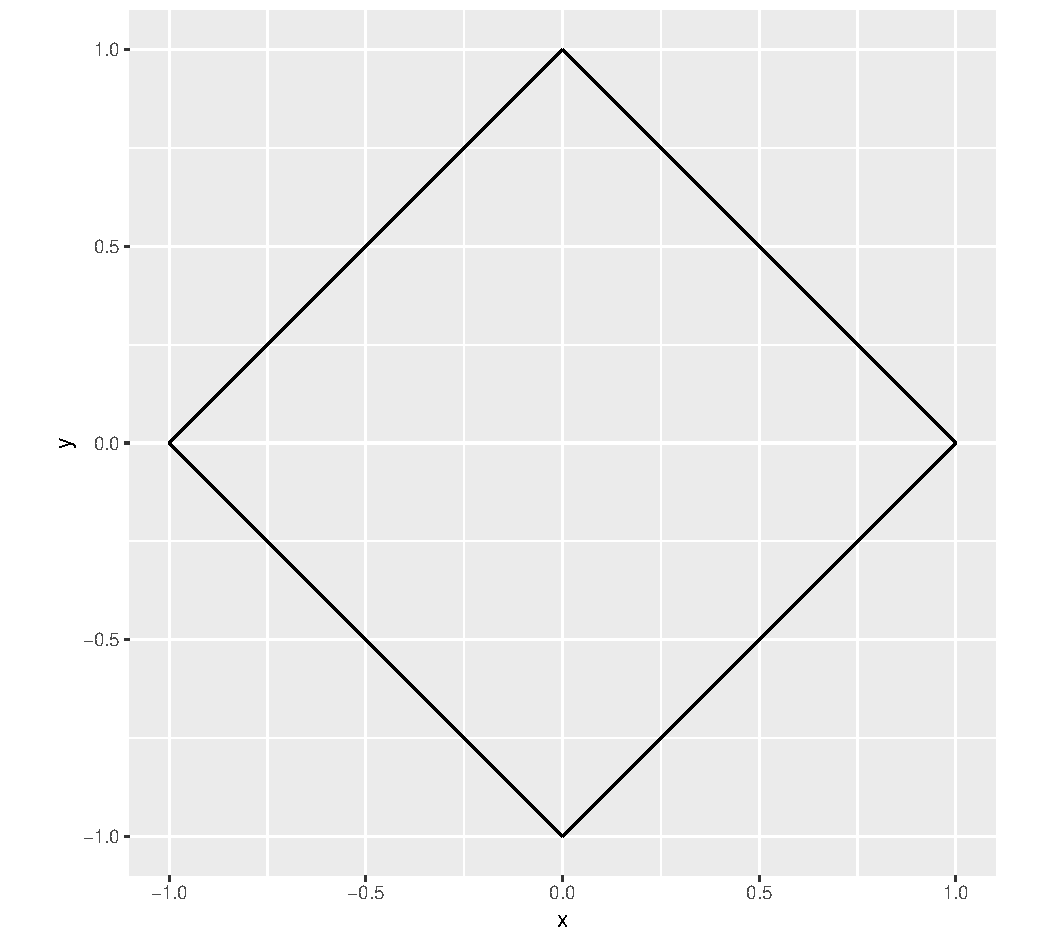
\includegraphics[width=0.3\textwidth]{unit_circle_1.pdf}
    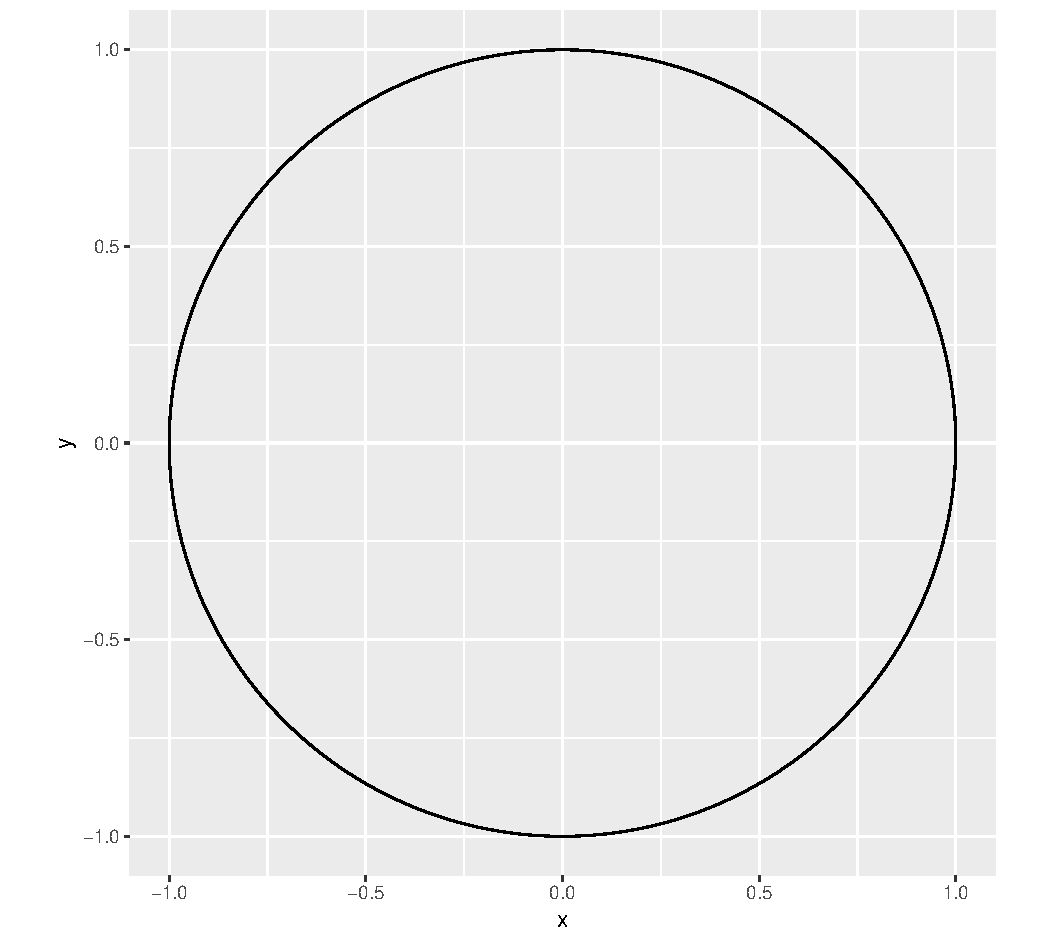
\includegraphics[width=0.3\textwidth]{unit_circle_2.pdf}
    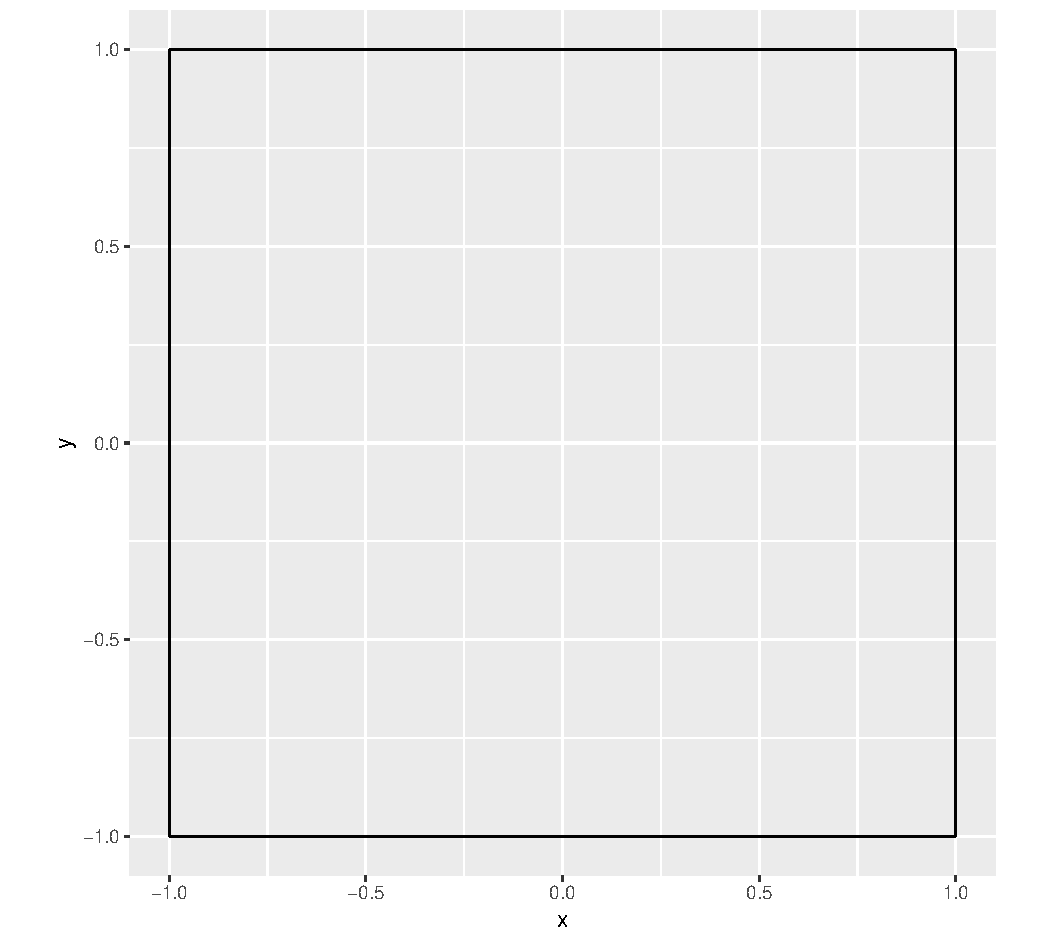
\includegraphics[width=0.3\textwidth]{unit_circle_inf.pdf}
    \caption{Unit balls in $\R^2$ of the $l_1$ (left), $l_2$ (center), an $l_\infty$ norm (right).}
    \label{fig:input}
\end{figure}
Note that for one-dimensional $x$, i.e.\ $x \in \R$, all $p$-norms conflate to the absolute value for $p > 0$.

\subsection{Example: $p$-Norm of a Vector}
The $5$ dimensional vector 
$$v = 
\begin{pmatrix}
1 \\ 1 \\ -3 \\ -5
\end{pmatrix}
$$
has $1$ norm
\begin{eqnarray*}
||v||_1 &=& \sum_{i = 1}^d |x_i| \\
&=& 1 + 1 + 3 + 5 \\
&=& 10,
\end{eqnarray*}
has $2$ norm
\begin{eqnarray*}
||v||_2 &=& \sqrt{\sum_{i = 1}^d x_i^2} \\
&=& \sqrt{1^2 + 1^2 + (-3)^2 + (-5)^2} \\
&=& \sqrt{36} \\
&=& 6,
\end{eqnarray*}
and $\infty$ norm
\begin{eqnarray*}
||v||_\infty &=& \max_i |x_i| \\
&=& \max(1, 1, 3, 5) \\
&=& 5.
\end{eqnarray*}

\section{Induced Vector Norms}
An induced vector norm is a function of an arbitrary vector $v \in \R^{n \times d}$ of the form
$$||v||_{p} = \sup_{\{x \in \R^d: ||x||_p \leq 1\}} |v^T x|,$$
where $|\cdot|$ denotes the absolute value, i.e. a $q$-norm with arbitrary $q > 0$.
Intuitively, the induced norm of a vector $v$ measures, or more precisely limits, how far it can project a vector $x$.
In order for this statement to make sense, we need to limit the size of applicable vectors $x$ by limiting the $q$ norm of $x$ to be 1 (note that the limitation $||x||_p \leq 1$ simplifies is in practice $||x||_p = 1$). 
The size of the projection $v^Tx$ is measured using the absolute value.

For some pairs of $p$ and $q$, the induced norm $||A||_{p \to q}$ is analytically directly accessible, see Table~\ref{tab:induced_v_norm}. 

\begin{table}[ht]
\caption{Analytically accessible induced vector norms $||v||_{p}$ for domain $p$.}
\begin{tabular}{ll|p{2.5cm}p{3cm}p{3.5cm}}
\multirow{4}{*}{p} &    & Induced norm & Maximizing input $\hat x$  & remarks on $\hat x$ \\ \cline{2-5}
    & 1 & $||v||_\infty$ & $e_i, \ i = \underset{j}{\text{arg max }} |v_j|$ &  $\hat x$ is one hot vector with 1 where $|v_i|$ is largest\\
    & 2 & $||v||_2$ & $\frac{1}{||v||_2} v$ &  $\hat x$ is scaled version of $v$\\
    & $\infty$ & $||v||_1$ & $\text{sign}(v)$ & $\hat x_i=
        \begin{cases}
        1 & v_i \leq 0 \\
        -1 & v_i < 0
        \end{cases}$  
\end{tabular}
\label{tab:induced_v_norm}
\end{table}

\subsection{Example: Induced Norm of a Vector of length 4}
To illustrate the induced norm consider the following vector
$$
v = \begin{pmatrix}
1 \\ 1 \\ -3 \\ -5 \\
\end{pmatrix}.$$

Its induced norms and maximizing input vector are given in Table~\ref{tab:example_induced_v_norm}.

\begin{table}[ht]
\caption{Analytically accessible induced vector norms $||v||_{p}$ for domain $p$.}
\begin{tabular}{ll|p{2.5cm}p{6.5cm}}
\multirow{4}{*}{p} &    & Induced norm & Maximizing input $\hat x$ \\ \cline{2-4}
    & 1 & $||v||_\infty = 5$ & $ (e_i, \ i = \underset{j}{\text{arg max }} |v_j|) = (0, 0, 0, 1)$ \\
    & 2 & $||v||_2$ = 6 & $\frac{1}{||v||_2} v = \frac{1}{6} (1, 2, -3, -5) = (\frac{1}{6}, \frac{1}{6}, -\frac{1}{2}, -\frac{5}{6})$ \\
    & $\infty$ & $||v||_1 = 10$ & $\text{sign}(v) = (1, 1, -1, -1)$   
\end{tabular}
\label{tab:example_induced_v_norm}
\end{table}


\section{Induced Matrix Norms}
An induced matrix norm is a function of an arbitrary matrix $A \in \R^{n \times d}$ of the form
$$||A||_{p \to q} = \sup_{\{x \in \R^d: ||x||_p \leq 1\}} ||Ax||_q.$$
Intuitively, the induced norm of a matrix $A$ measures, or more precisely limits, how far it can distort a vector $x$.
In order for this statement to make sense, we need to limit the size of applicable vectors $x$ by limiting the $p$ norm of $x$ to be 1 (note that the limitation $||x||_p \leq 1$ simplifies is in practice $||x||_p = 1$). 
The size of the "distorted $x$" $Ax$ is measured using the $q$ norm.
A common notational shorthand when $p = q$ is to write
$$||A||_p = ||A||_{p \to p}.$$

For some pairs of $p$ and $q$, the induced norm $||A||_{p \to q}$ is analytically directly accessible, see Table~\ref{tab:induced_norm}. 

\begin{table}[ht]
\caption{Analytically accessible induced norms $||A||_{p \to q}$ for domain $p$ and co-domain $q$. NP hard stands for "non-deterministic polynomial-time hardness" which means not computable for our purposes.}
\begin{tabular}{ll|p{3cm}p{3cm}p{3cm}}
                          & & \multicolumn{3}{l}{\hspace{5cm} q} \\ 
\multirow{4}{*}{p} &                       & 1 & 2  & $\infty$ \\ \cline{2-5}
                          & 1 & max $l_1$ norm of a column & max $l_2$ norm of a column & max $l_\infty$ norm of a column \\
                          & 2                     & NP-hard & max singular value  & max $l_2$ norm of a row \\
                          & $\infty$ & NP-hard & NP-hard & max $l_1$ norm of a row     
\end{tabular}
\label{tab:induced_norm}
\end{table}


\subsection{Example: Induced Norm of a $2 \times 2$ matrix}
In order to get a better handle on this theoretical concept, consider the induced norm of the following matrix 
$$A = 
\begin{pmatrix}
1 & 3 \\
2 & 1
\end{pmatrix}.$$

The applicable input vectors $\{x \in \R^d: ||x||_p = 1\}$ for the $||\cdot||_p = 1, 2$ and $\infty$ norm, are depicted in Figure~\ref{fig:input}. All $x$ on the unit circle have $||x||_p = 1,$ for $p = 1, 2, \infty$ respectively. Note that the applicable input vectors $x$ are \textbf{not} specific to the choice of $A$ but only to the choice of the $p$.
In order to find the supremum over all applicable input vectors, all applicable $x$ are  multiplied by $A$. The points $Ax$ are depicted in Figure~\ref{fig:output}. The induced norm is defined as the maximum $q$ norm of all points $\{Ax\}$.



\begin{figure}[ht]
    \centering
    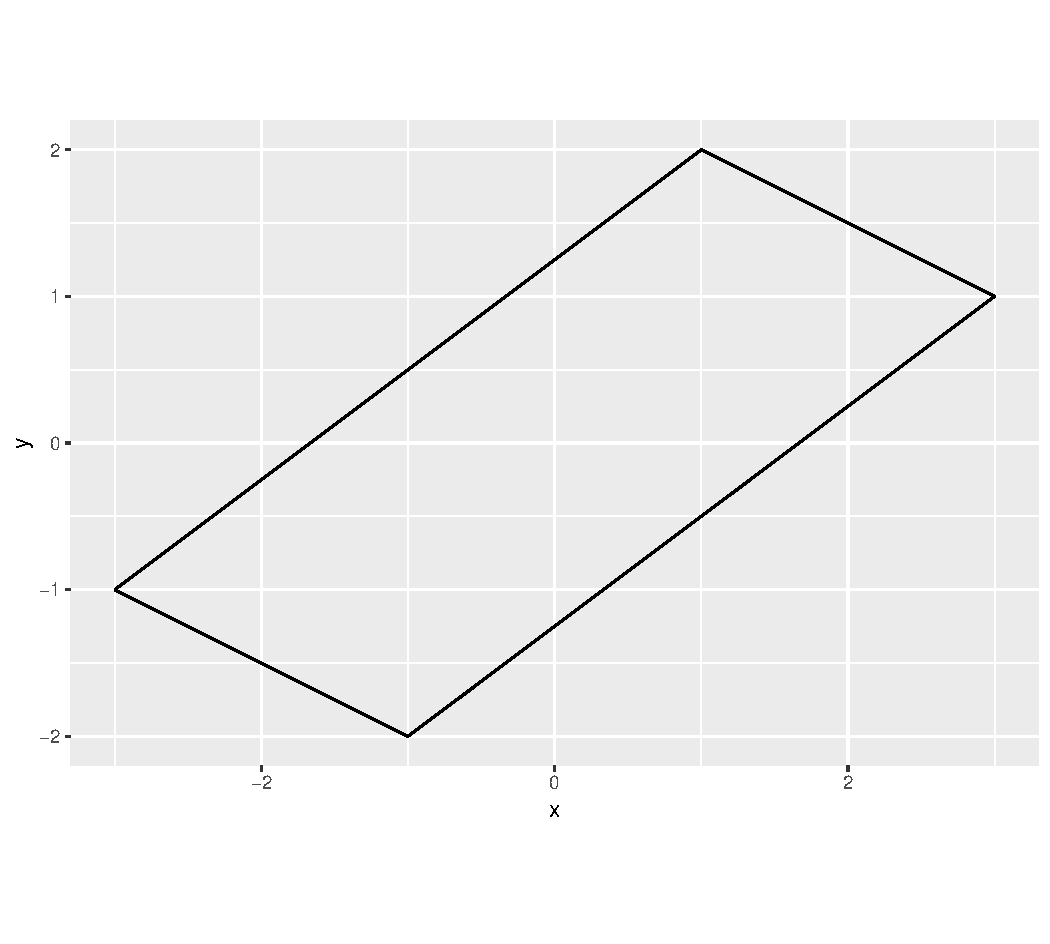
\includegraphics[width=0.3\textwidth]{A_unit_circle_1.pdf}
    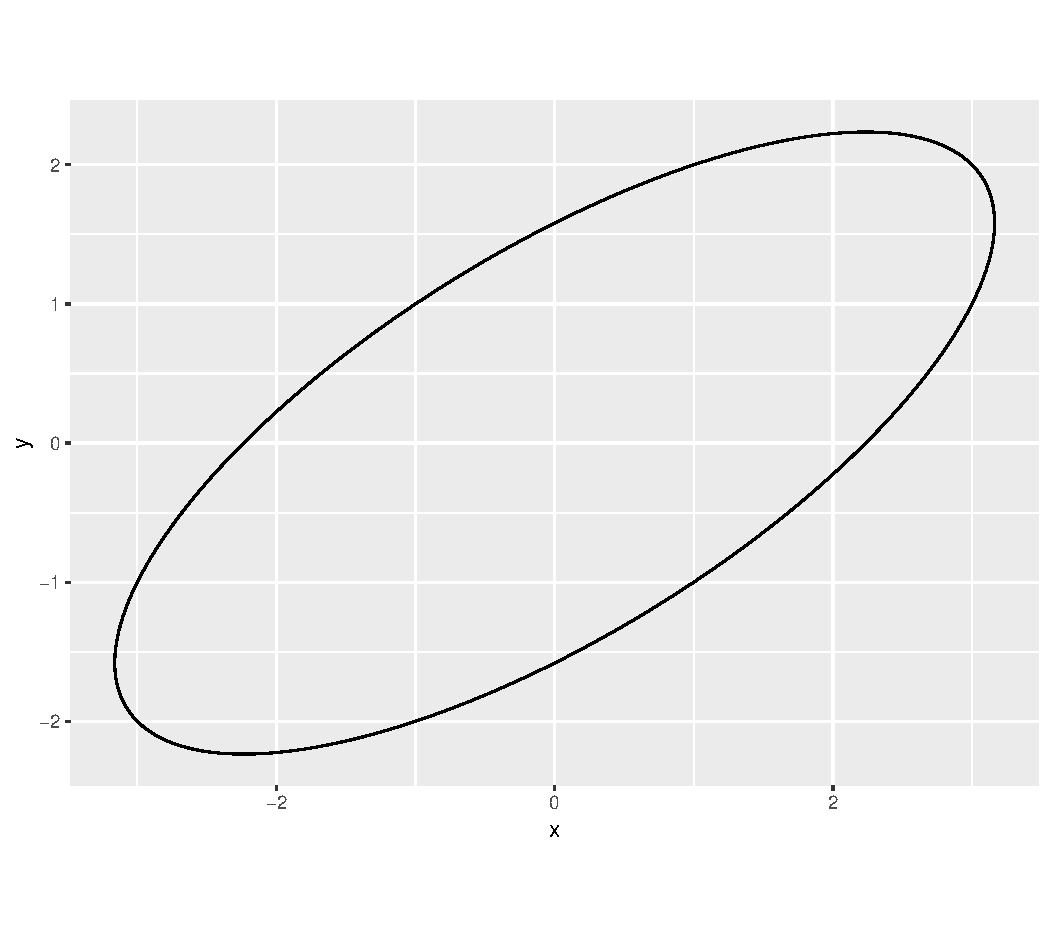
\includegraphics[width=0.3\textwidth]{A_unit_circle_2.pdf}
    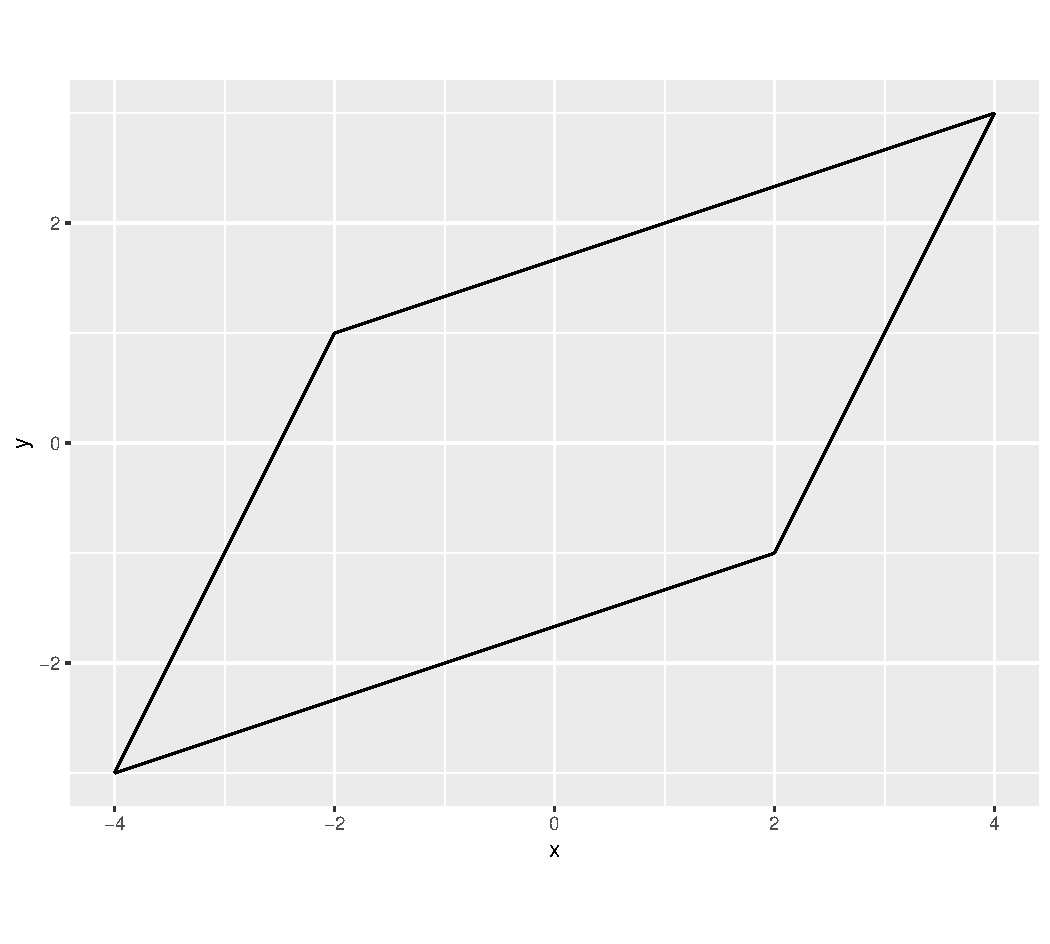
\includegraphics[width=0.3\textwidth]{A_unit_circle_inf.pdf}
    \caption{Projection of the unit circles by $A$, i.e. $Ax$ for every point $\{x \in \R^d: ||x||_p = 1\}$ for $p = 1$ (left), $p = 2$ (center), and $p = \infty$ (right).}
    \label{fig:output}
\end{figure}

\begin{figure}[ht]
    \centering
    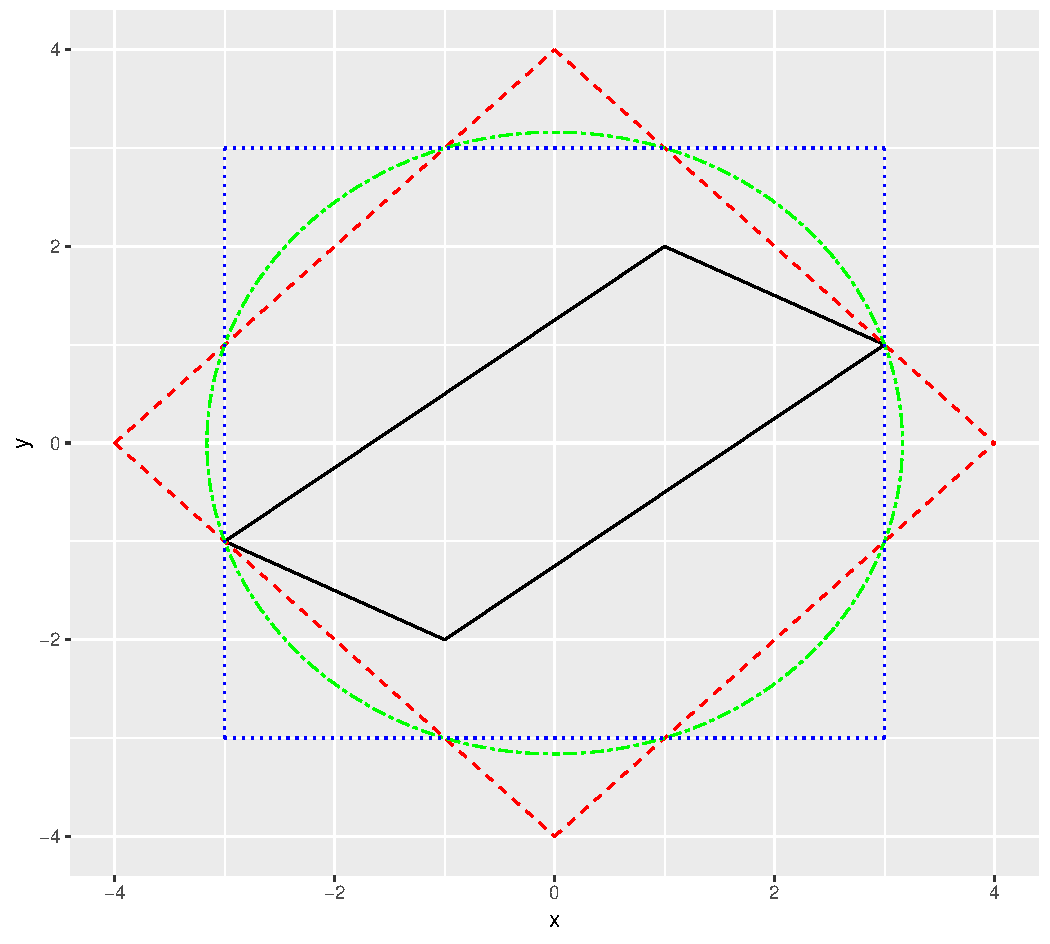
\includegraphics[width=0.3\textwidth]{norms_A_unit_circle_1.pdf}
    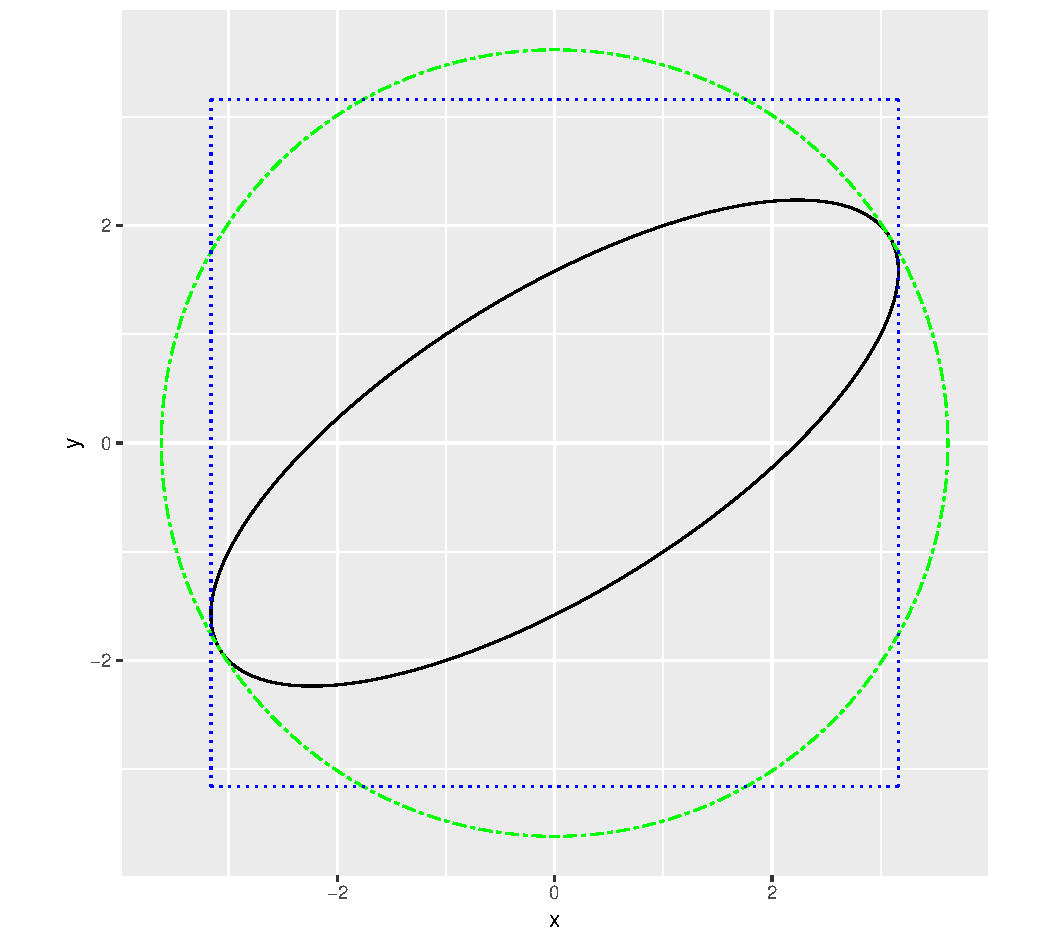
\includegraphics[width=0.3\textwidth]{norms_A_unit_circle_2.pdf}
    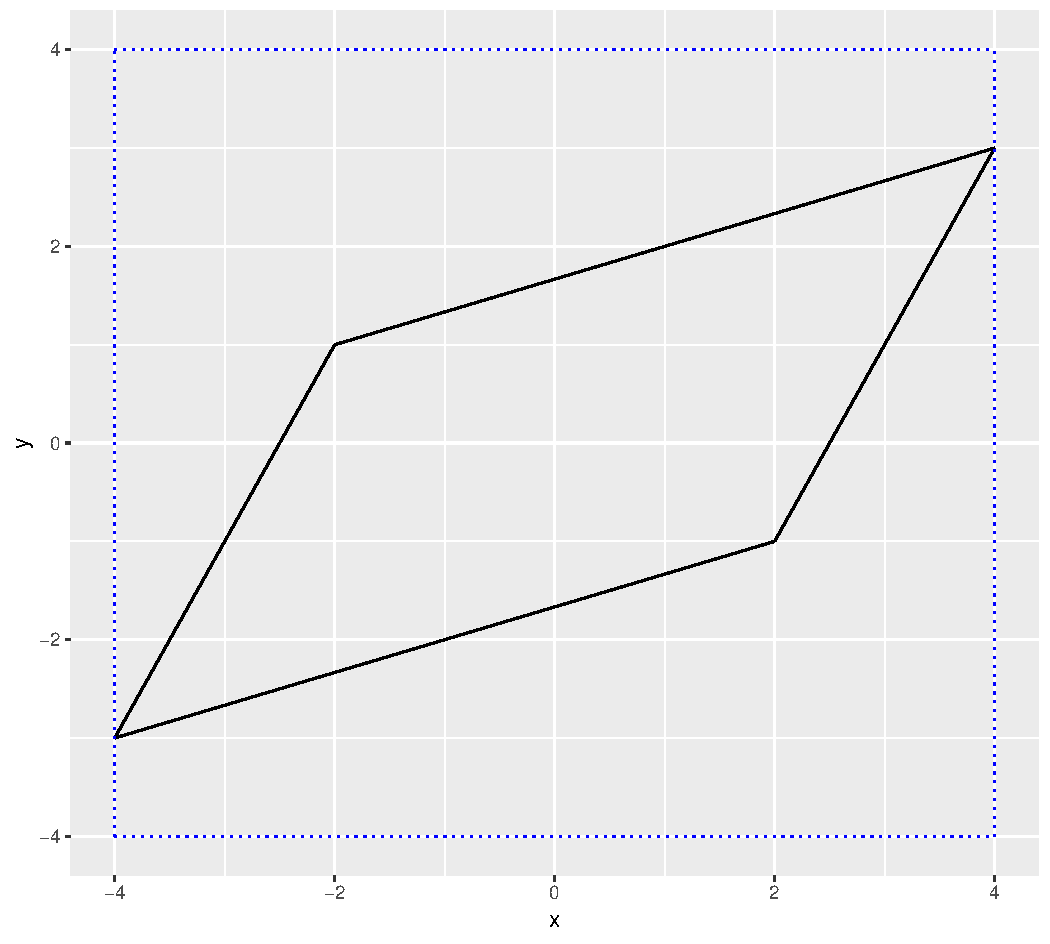
\includegraphics[width=0.3\textwidth]{norms_A_unit_circle_inf.pdf}
    \caption{The colored circles are unit circles of size $||A||_{p \to q}$ for every point $x, ||x||_p = 1$ with p = 1 (left), $p = 2$ (center), an $p = \infty$ (right). 
    The $1$ norm is depicted in red, the $2$ norm in green, and the $\infty$ norm in blue.
    Induced norms that are hard to compute were omitted.}
    \label{fig:norms_output}
\end{figure}

We can use Table~\ref{tab:induced_norm} to compute $||||A||_{p \to q}$ for some combinations of $p$ and $q$, see values reported in Table~\ref{tab:example_induced_norms}. Figure~\ref{fig:norms_output} shows $Ax$ with $q$-norm circles of radius $||A||_{p \to q}$ around the origin. The intersection of the $q$ norm circles with $Ax: ||x||_p = 1$ shows which $Ax$ achieves the induced norm, i.e. the $\sup_x ||Ax||_q$.


\begin{table}[ht]
\caption{Analytically accessible results $||A||_{p \to q}$ for our example. These values match up with the size of the colored circles in Figure~\ref{fig:norms_output}.}
\begin{tabular}{ll|p{3cm}p{3cm}p{3cm}}
                          & & \multicolumn{3}{l}{ \hspace{5cm} q} \\ 
\multirow{4}{*}{p} &                       & 1 & 2  & $\infty$ \\ \cline{2-5}
                          & 1 & $\max(|1| + |3|, |1| + |2|) = 4$ & $\max(\sqrt{10}, \sqrt{5}) \approx 3.16$ & $\max(|3|, |2|) = 3$ \\
                          & 2                     & NP-hard & $\sigma_\text{max} \approx 3.62$  & $\max(\sqrt{10}, \sqrt{5}) \approx 3.16$ \\
                          & $\infty$ & NP-hard & NP-hard & $\max(|1| + |3|, |1| + |2|) = 4$    
\end{tabular}
\label{tab:example_induced_norms}
\end{table}


\end{document}